\documentclass[../../thesis.tex]{subfiles}

\begin{document}

Our work, as well as out models can be divided into two stages. Firstly we investigate the effect of non-contrastive SSL on a proven tokenization model, VQVAE \cite{VQVAE}, with the goal of learning more expressive representations. The expressiveness is measured in terms of the models ability to reconstruct unseen data, as well at the performance of learned latent representations on a downstream classification task. The SSL models we consider are, as introduced in section 2 \todo{make hyperlink}, BarlowTwins, VIbCReg and BYOL.\\\\

Secondly we investigate the effects of SSL-VQ-VAE on prior learning by training a MaskGIT model on top of the tokenization models.


\begin{figure}[h]
    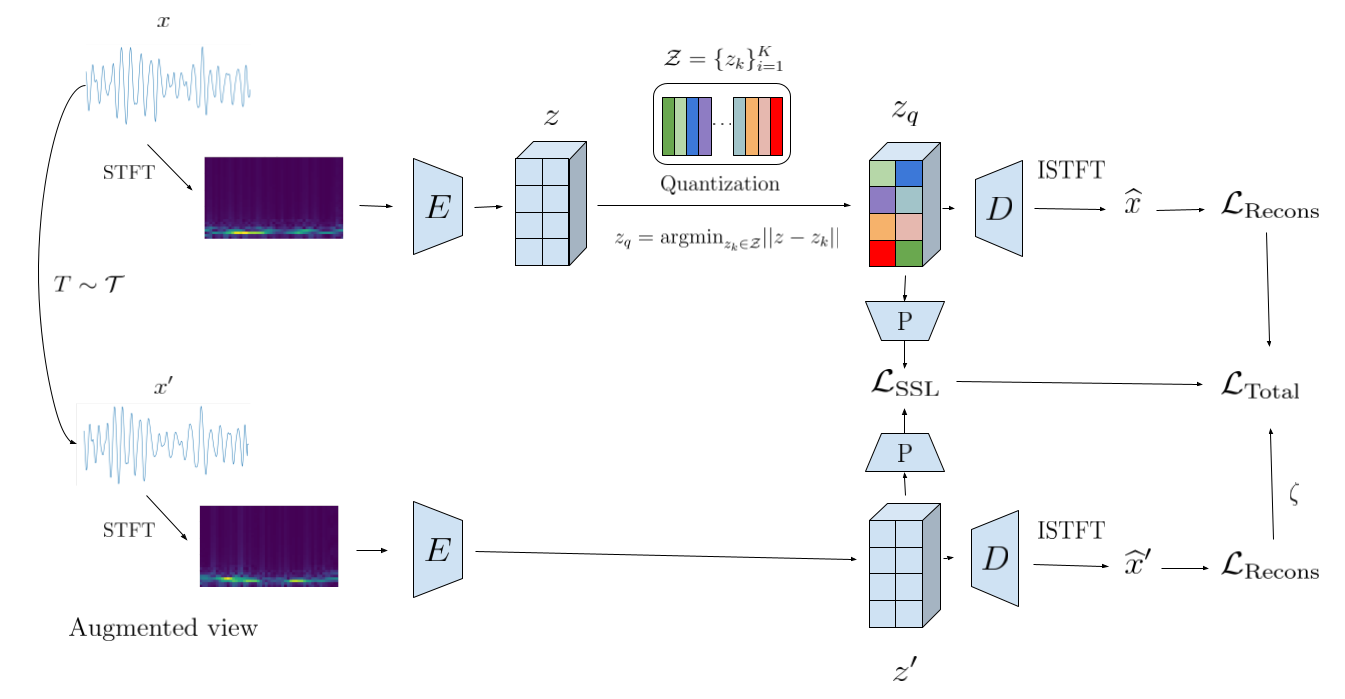
\includegraphics[scale=0.5]{Siam-VQVAE.png}
    \centering    
\end{figure}


\section{Stage 1}
We compare the latent representations learned from basic TimeVQVAE with a Barlow Twins extended version on downstream tasks as classification and reconstruction.



\subsection{VQ-VAE}
The VQ-VAE model is baseline for our experiments.\\

An encoder, decoder, and codebook are to be optimized by compressing the input into discrete latent space, minimizing information loss by comparing input to the output, which ideally are equal. We follow \cite{TimeVQVAE} and augment time-series into time-frquency domain, but leave the high-low frequency split for future work. \\

\subsubsection{Model Architecture}
A schematic overwiew of the VQ-VAE model is presented in "Figure here"

A time series is first augmented into time-frequency domain using the Short-time Fourier Transform (cite pytorch stft). Then it is encoded into the continious latent space, and is discretized by the codebook via the argmin process. In the argmin process the continious token is compared to every discrete token in the codebook, and replaced by the closes discrete token in terms of euclidean distance. Then, the decoder maps the discrete token back to time-frequency domain, before finally being mapped back to time domain using the ISTFT.



\subsection{Barlow Twins VQ-VAE}
\subsubsection{Model Architecture}


An encoder, decoder, codebook, and projector are to be optimized.

Produce two augmented views of the time-series, augment views into time-frequency domain and encode into latent space. Choose one view for quantization, decoding and comparrison to original time series (VQVAE loss). Project both latent embeddings and calculate Barlow loss. Update using both VQVAE and Barlow loss.

A schematic overwiew of the BT-VQ-VAE model is presented in "Figure here"

\subsection{VIbCReg VQ-VAE}

\subsubsection{Augmentations}
We used the following collection of augmentation techniques throughout. Never dataset specific.
\begin{itemize}
    \item Flip
    \item Jitter
    \item Amplitude Resizing
    \item Adding slope
    \item STFT Augmentation
\end{itemize}

\subsubsection{Model Architecture}

\subsubsection{Training}

\section{Stage 2}

\subsection{MaskGIT}

\end{document}